% Simplified method-flow figure.
% Shows ONLY the executed artifact path (no multi-agent, no ground control,
% no closed update loop, no RL claim).
% Requires tikz + arrows.meta + positioning
% (tikz and positioning are loaded by Definitions/mdpi).

% (tikz itself is loaded by Definitions/mdpi; the libraries are pulled in here
%  so this file compiles standalone as well as inside the MDPI class.)
\usetikzlibrary{arrows.meta,positioning,calc}

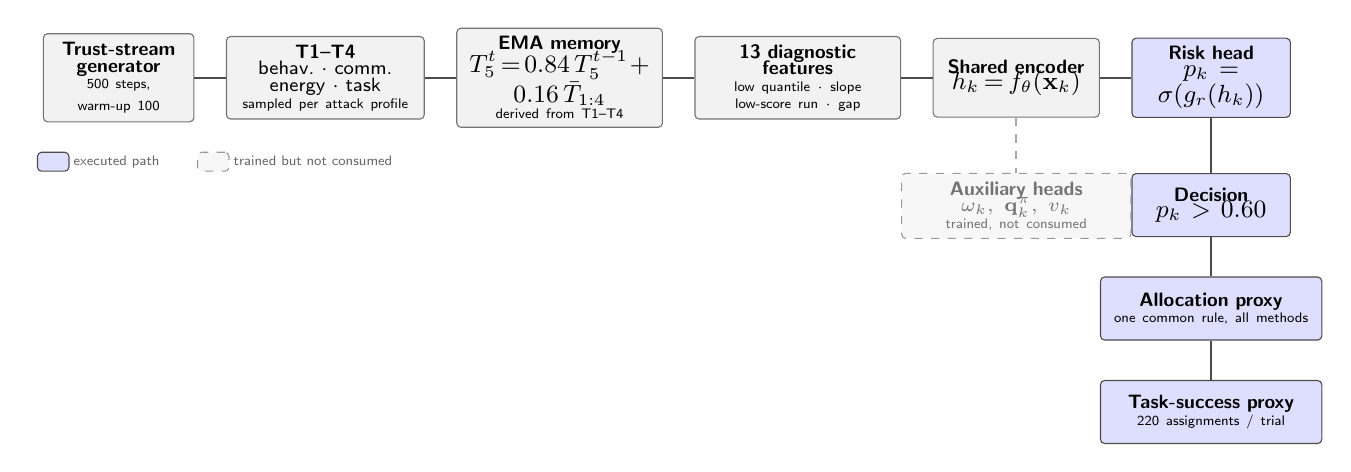
\begin{tikzpicture}[
  font=\sffamily\scriptsize,
  >=Stealth,
  node distance=4mm,
  line/.style={draw=black!70, line width=0.6pt},
  ghostline/.style={draw=black!35, line width=0.6pt, dashed},
  stage/.style={draw=black!55, fill=black!5, rounded corners=1.5pt, align=center,
                minimum height=10mm, inner xsep=3pt, inner ysep=3pt},
  used/.style={draw=black!70, fill=blue!13, rounded corners=1.5pt, align=center,
               minimum height=8mm, inner xsep=3pt, inner ysep=3pt},
  unused/.style={draw=black!40, fill=black!3, dashed, rounded corners=1.5pt, align=center,
                 minimum height=8mm, inner xsep=3pt, inner ysep=3pt, text=black!55},
  tag/.style={font=\sffamily\tiny, text=black!60, align=center}
]

% ============ Row 1: evidence generation -> encoding -> risk ============
\node[stage, text width=17mm] (gen) {
  \textbf{Trust-stream}\\[-2pt]\textbf{generator}\\[-2pt]{\tiny 500 steps, warm-up 100}};

\node[stage, right=of gen, text width=23mm] (t14) {
  \textbf{T1--T4}\\[-2pt]behav.\ $\cdot$ comm.\\[-2pt]energy $\cdot$ task\\[-2pt]{\tiny sampled per attack profile}};

\node[stage, right=of t14, text width=24mm] (t5) {
  \textbf{EMA memory}\\[-2pt]{\small $T_5^{t}\!=\!0.84\,T_5^{t-1}\!+\!0.16\,\bar{T}_{1:4}$}\\[-2pt]{\tiny derived from T1--T4}};

\node[stage, right=of t5, text width=24mm] (feat) {
  \textbf{13 diagnostic}\\[-2pt]\textbf{features}\\[-2pt]{\tiny low quantile $\cdot$ slope}\\[-2pt]{\tiny low-score run $\cdot$ gap}};

\node[stage, right=of feat, text width=19mm] (enc) {
  \textbf{Shared encoder}\\[-2pt]{\small $h_k\!=\!f_\theta(\mathbf{x}_k)$}};

\node[used, right=of enc, text width=18mm] (risk) {
  \textbf{Risk head}\\[-2pt]{\small $p_k\!=\!\sigma(g_r(h_k))$}};

\draw[line] (gen) -- (t14);
\draw[line] (t14) -- (t5);
\draw[line] (t5)  -- (feat);
\draw[line] (feat) -- (enc);
\draw[line] (enc)  -- (risk);

% ============ Evaluated decision path ============
\node[used, below=7mm of risk, text width=18mm] (dec) {
  \textbf{Decision}\\[-2pt]{\small $p_k>0.60$}};
\node[used, below=5mm of dec, text width=26mm] (alloc) {
  \textbf{Allocation proxy}\\[-2pt]{\tiny one common rule, all methods}};
\node[used, below=5mm of alloc, text width=26mm] (tsr) {
  \textbf{Task-success proxy}\\[-2pt]{\tiny 220 assignments / trial}};

\draw[line] (risk) -- (dec);
\draw[line] (dec)  -- (alloc);
\draw[line] (alloc) -- (tsr);

% ============ Auxiliary head, off the evaluated path ============
\node[unused, below=7mm of enc, text width=27mm] (aux) {
  \textbf{Auxiliary heads}\\[-2pt]$\mathbf{\omega}_k,\ \mathbf{q}_k^{\pi},\ v_k$\\[-2pt]{\tiny trained, not consumed}};
\draw[ghostline] (enc) -- (aux);

% ============ Legend ============
\node[tag, anchor=west] at ([xshift=-2mm,yshift=-5mm]gen.south west) {
  \tikz[baseline=-0.6ex]\node[used, minimum height=2.4mm, minimum width=4mm, inner sep=0pt] {};\hspace{1.5pt}executed path
  \hspace{10pt}
  \tikz[baseline=-0.6ex]\node[unused, minimum height=2.4mm, minimum width=4mm, inner sep=0pt] {};\hspace{1.5pt}trained but not consumed
};

\end{tikzpicture}
